
\chapter{Team software development}

At some point in your career (perhaps now), you will begin to work on projects
that are too big for any one person to complete in an acceptable amount of
time. The solution, of course, is to work on a \textbf{team} with other
software developers. Working on a team brings up a host of other issues, some
technical and some social.

\section{Team-based version control with \texttt{git}}

\index{git@\texttt{git}}
\index{CLI (command-line interface)}
Waaaay back in \chapref{ch:gettingOff} (p.~\pageref{introduceGit}) I briefly
introduced the \texttt{git} version control system. Hopefully you've been
using it all along to do the simple process of ``committing'' code to your
repo in individual snapshots. This is a habit you'll want to continue to
ingrain in your cerebral cortex. Commits are the building blocks of any
version control system, including \texttt{git}; without them, you don't have
anything to work with.

Now it's time to learn a little more about \texttt{git}, and especially how it
works in a team environment.

\index{repository@``repo'' (repository)}
\index{directory!child}
\index{bleeding edge}
\index{workspace}
\index{vim@\texttt{vim}}
\index{Filbert}
\index{tree}
Figure~\ref{fig:filbertGit} shows the environment you've been using so far: a
single developer, with a single \textbf{repo}. I use the term
\textbf{workspace} to mean ``the directory (and possibly subdirectories) in
which the developer's files actually exist.'' In Figure~\ref{fig:filbertGit},
the developer is Filbert. His workspace is shown as a yellow oval, which
matches the ovals from way back in Figure~\ref{fig:tree}
(p.~\pageref{fig:tree}) that represented ordinary Linux directories. This
yellow oval contains the ``bleeding edge'' of what Filbert is working on: as
soon as he saves any file from \texttt{vim}, the file in that directory is
instantly updated based on what he just typed, warts and all.

\begin{figure}[ht]
\centering
\includegraphics[width=0.4\textwidth]{filbertGit.pdf}
\caption{A single developer's repo and workspace.}
\label{fig:filbertGit}
\end{figure}

\index{git@\texttt{git}!\texttt{.git} directory}
\index{cd@\texttt{cd}}
Filbert's personal git repo is shown as a green box. At this point, you should
view a repo as a sort of ``mysterious'' thing that somehow maintains a record
of all the previous changes to all the project's files, yet in a way you don't
need to understand. Using \texttt{git} commands from the command line is the
only way we will inspect and command it.\footnote{If you're curious, it is
maintained in a hidden directory called ``\texttt{.git}'' -- note the initial
dot -- inside the top-level directory of your workspace. If you \texttt{cd} in
there, you'll see all kinds of crazy stuff under the hood. Do \textit{not}
modify any of it, or you'll probably break your repo and lose all its contents!}

\index{staging area}
\index{git@\texttt{git}!\texttt{git status}}
\index{git@\texttt{git}!\texttt{git add}}
\index{git@\texttt{git}!\texttt{git commit}}
\index{commit}
Also shown is a purple diamond called the \textbf{staging area}. Normally you
don't think too hard about the purple diamond explicitly, but it is there, and
the command ``\texttt{git status}'' will only fully make sense if you recognize
its use. Essentially, the staging area is for changes that the developer is
``about to commit'' (or ``fixin' to commit,'' as they sometimes say in the
South) but hasn't actually pulled the trigger on yet. When you execute the two
commands ``\texttt{git add}'' and ``\texttt{git commit}'', back to back, the
\texttt{add} puts a snapshot of the change to the staging area, and
\texttt{commit} actually records it in the repo. If you're in the habit of
using ``\texttt{git commit -a}'' to commit your files, it effectively does both
the add and the commit all in one step.

\label{commitPitfall}
Beware a common pitfall with ``\texttt{git commit -a}'', though: it only
commits changes to \textit{existing} files, not \textit{new} files. If you
create a brand new \texttt{.java} file in your workspace, representing a new
class, you must explicitly ``\texttt{git add}'' it to your repo before
committing it. I can't tell you how many times one of my colleagues (or myself
*shame*) has broken a build by committing all of their changes \textit{except}
for the new files.

Anyway, just to repeat the basic instructions for reproducing
Figure~\ref{fig:filbertGit}:

\index{mkdir@\texttt{mkdir}}
\index{hairball}
\begin{compactenum}
\item The command ``\texttt{mkdir someDirectoryName}'' creates the workspace,
under whatever directory you're currently in (which can be seen via
``\texttt{pwd}'').
\item The command ``\texttt{cd someDirectoryName}'' actually goes into that
directory (remember that \texttt{mkdir} alone does \textit{not} change your
current directory).
\item The command ``\texttt{git init .}'' creates the green box and the purple
diamond.
\item You use ``\texttt{vim}'' to create/edit files like \texttt{Cat.java} and
\texttt{Hairball.java} directly in your workspace (blue rectangles).
\item When you want to snapshot the current version of one of your files, in
anticipation of doing a commit, you type ``\texttt{git add nameOfFile}''. This
adds the current contents to the purple diamond. You can now proceed editing
further, or go straight to the commit.
\item To actually commit, type ``\texttt{git commit}'', enter a comment in the
editor, and quit the editor.
\end{compactenum}

\subsection{Understanding \texttt{git status}}

Two extremely common commands for inspecting your workspace are ``\texttt{git
status}'' and ``\texttt{git log}''. Let's look at each in turn.

\index{git@\texttt{git}!\texttt{git status}}
The \texttt{git status} command tells you the current state of your workspace
as compared with your repo. The output might look something like this:

\begin{Verbatim}[fontsize=\footnotesize,samepage=true,frame=single]
$ git status
On branch master
Changes to be committed:
  (use "git reset HEAD <file>..." to unstage)
    modified:   Cat.java

Changes not staged for commit:
  (use "git add <file>..." to update what will be committed)
  (use "git checkout -- <file>..." to discard changes in working directory)
    modified:   Cat.java

Untracked files:
  (use "git add <file>..." to include in what will be committed)
    Cat.class
    Hairball.class
    Hairball.java
\end{Verbatim}

\pagebreak
Several things of interest here:

\begin{itemize}

\index{branch}
\item The ``\texttt{On branch master}'' means you're on the main, default code
``trunk.'' Later in your career, you'll discover that you sometimes want to
create \textbf{branch}es, which are independently developed sequences of
changes for some specific purpose. They are normally brought back together and
merged into the trunk at a later time.

\item The output lists \texttt{Cat.java} as a ``change to be committed.'' This
means that an updated version of \texttt{Cat.java} is \textit{in your purple
diamond.} If we were to follow up this command with a ``\texttt{git commit}'',
that version of \texttt{Cat.java} would be committed to the repo for
posterity.

\item Somewhat weirdly, the output shows \texttt{Cat.java} as being in the
``changes \textit{not} staged for commit'' section as well! What the heck is
going on here -- is \texttt{Cat.java} going to be committed, or not?

The answer to that question is ``both.'' When a file shows up in both lists,
it means there have been several \textit{different} changes to it, only
\textit{some} of which were present the last time a ``\texttt{git add}'' was
performed, and which are therefore in the purple box. Other changes to this
same file were made \textit{after} the ``\texttt{git add}'', and so they are
in the yellow oval only. In a moment, I'll teach you how to find out which
changes are in which category. For now, just grasp the fact that the same file
can be in both sections of the ``\texttt{git status}'' output.

\index{untracked file}
\index{file!untracked}
\item The ``untracked'' files are the files in your workspace that
\texttt{git} doesn't yet know about. Looking at this list is a good way to
avoid making the ``oops I did a \texttt{git commit -a} but forgot to add my
new files'' problem I mentioned earlier (p.~\pageref{commitPitfall}). In this
case, \texttt{Hairball.java} is potentially such a file, and this message
reminds us that we may want to ``\texttt{git add}'' it. If we don't, our next
commit will \textit{only} have the (first set of) \texttt{Cat} changes, not
the \texttt{Hairball} changes.

\index{java file@\texttt{.java} file}
\index{class file@\texttt{.class} file}
\index{git@\texttt{git}!\texttt{.gitignore} file}
\item The other entries under ``untracked'' are compiled \texttt{.class}
files, not \texttt{.java} source files. \textbf{Normally, we \textit{want}
those to be untracked}, and so it's actually good that they're not set up as
part of the commit. Some developers, however (myself included) find this
message annoying. The way to fix it is to create a (hidden) file in your
project directory called ``\texttt{.gitignore}''. \textit{All files whose names
match something in the ``\texttt{.gitignore}'' file will be ignored entirely by
\texttt{git}}, and hence not be mentioned in a cries-wolf warning message.

\begin{samepage}
Here's an example \texttt{.gitignore} file, which you can edit like any other
file in \texttt{vim}:

\begin{Verbatim}[fontsize=\small,samepage=true,frame=single]
.gitignore
*.class
\end{Verbatim}
\end{samepage}

There are two lines. The first is a bit of a mind-blower: it's the name of the
\texttt{.gitignore} file itself! By including the line ``\texttt{.gitignore}''
in our \texttt{.gitignore}, we're telling \texttt{git} to not do version
control on \texttt{.gitignore} itself. (Without that, we'll feel like we're
stuck in a Monty Python skit where we create a \texttt{.gitignore} to avoid
annoying warning messages, only for the \texttt{.gitignore} file itself to
cause another annoying warning message.)

The second line says ``also please ignore any file that ends with
\texttt{.class}''. Now, we know that anything that shows up in the ``untracked
files'' section of \texttt{git status} really is something to think hard about.

\item Finally, notice the helpful comments that ``\texttt{git status}''
provides: they're great for telling you exactly how to change things if
necessary. For instance:

\begin{compactitem}

\index{git@\texttt{git}!\texttt{git reset}}
\index{git@\texttt{git}!\texttt{git checkout}}
\item If we decide we don't want to check in that first set of
\texttt{Cat.java} changes after all, we run the command ``\texttt{git reset
HEAD Cat.java}'' to remove it from the purple diamond.

\item If we want \textit{all} our changes in \texttt{Cat.java} to be committed
(the old pre-\texttt{-git-add} ones and the newer ones), we do ``\texttt{git
add Cat.java}'' which will update the purple diamond's copy to match the
workspace.

\item If we decide to actually ditch the \texttt{Cat.java} changes entirely,
the command is ``\texttt{git checkout -{}- Cat.java}'' to discard them.
(Notice the double-hyphen, and also the spaces on either side of it: it's a
weird syntax but you have to use it.)

\end{compactitem}

\end{itemize}

\subsection{Understanding \texttt{git log}}

\index{git@\texttt{git}!\texttt{git log}}
While \texttt{git status} is a detailed look at the present, ``\texttt{git
log}'' is a detailed look at the \textit{past}. With it, we can see the time,
author, and description of every change that's been made during our whole
project.

I personally find the default \texttt{git log} output pretty wordy. It uses
multiple lines per commit, which to me is TMI and fills up my screen too
quickly:

\begin{Verbatim}[fontsize=\footnotesize,samepage=true,frame=single]
$ git log
commit 928ab4924f1c5ddd3b9e2a1c7b507b1b60cf745d
Author: Betty Lou <bettylou@umw.edu>
Date:   2018-11-03

    Fix NPE bug caused by multiple hairballs.

commit 7813b199f40051df14b23a418bce37ccb51a986d
Author: Filbert <filbert@umw.edu>
Date:   2018-11-02

    Add support for multiple, simultaneous hairballs.

commit bdb0fa3071a220bfaccb0d687046e73873a6381d
Author: Betty Lou <bettylou@umw.edu>
Date:   2018-10-21

    Make most setters private.

commit e4471910b8d27c819e4e0df39804ab607cd16c5c
Author: Jezebel <jezebel@umw.edu>
Date:   2018-10-15

    Add Cat.java, Hairball.java.
\end{Verbatim}

\index{hash}
\index{commit hash}
Notice that the entries are in reverse-chronological order (most recent at the
top), which is what you want to get used to. Each five-line section represents
one commit. The big hairy numbers immediately after the word \texttt{commit}
are called the commit's \textbf{hash}. That just means that every commit has a
unique number, randomly/automatically generated by \texttt{git}, so that you
can unambiguously refer to it. (More on why to do this in a moment.)

The \texttt{Author} and \texttt{Date} elements are self-explanatory, and the
rest of the text is the actual message that the developer typed when doing the
\texttt{git commit}.

It turns out that \texttt{git} provides a great deal of fine-grained control
over what this output looks like. (Right away, that tells you that people look
at git logs a \textit{lot} and need them to be just the right format to
quickly cull maximum information from them.) I like mine to be all on one
line, and in color. To do this, I execute the line:

\begin{Verbatim}[fontsize=\footnotesize,samepage=true,frame=none]
$ git config --global format.pretty "(%h) %Cblue%an%Creset: %Cgreen%s %Creset(%ad)"
\end{Verbatim}

which looks bizarre, but there's a method to its madness. Each one of these
control characters (starting with a ``\texttt{\%}'') specifies a certain piece
of information or formatting. The result, when I type \texttt{git log} is
this:

\definecolor{darkgreen}{rgb}{0,.65,0}
\begin{Verbatim}[commandchars=\\\{\},fontsize=\footnotesize,samepage=true,frame=single]
$ git log
(928ab49) \textcolor{blue}{Betty Lou}: \textcolor{darkgreen}{Fix NPE bug caused by multiple hairballs.} (2018-11-03)
(7813b19) \textcolor{blue}{Filbert}: \textcolor{darkgreen}{Add support for multiple, simultaneous hairballs.} (2018-11-02)
(bdb0fa3) \textcolor{blue}{Betty Lou}: \textcolor{darkgreen}{Make most setters private.} (2018-10-21)
(e447191) \textcolor{blue}{Jezebel}: \textcolor{darkgreen}{Add Cat.java, Hairball.java.} (2018-10-15)
\end{Verbatim}

\index{man@\texttt{man}}
Easier on the eyes, IMO. Run the command ``\texttt{man git config}'' to see
all the options. Btw, you may be wondering what good it does to only list the
first few characters of the commit hash. It turns out that for most commands
that use it, you only have to type the first few characters anyway (just
enough to guarantee uniqueness) and the short version is waaaay easier to look
at.

\subsection{Comparing versions}

\index{diff@\texttt{diff}}
A very common operation for a developer is to compare two versions (of the
code base, or of a single file) to see what changed between them.
Colloquially, comparing two versions of something is called ``\textbf{doing a
diff},'' named after the Linux ``\texttt{diff}'' command. Here's my favorite
way of comparing versions.

\subsubsection{The \texttt{vimdiff} comparison tool}

\index{vimdiff@\texttt{vimdiff}}
\index{git@\texttt{git}!\texttt{git config}}
First, make these changes to your \texttt{git} profile\footnote{By the way,
any time you want to see \textit{all} of your \texttt{git} configuration
settings, you can do so with the command ``\texttt{git config -e -{}-global}''.
It will bring up all your settings in a text file for you to browse in
\texttt{vim}. You can even edit this file directly to make changes to
settings, although be very careful not to mistype anything. Stuff can go
haywire if you do!}:

\begin{Verbatim}[fontsize=\small,samepage=true,frame=none]
$ git config --global merge.tool vimdiff
$ git config --global diff.tool vimdiff
$ git config --global difftool.prompt false
\end{Verbatim}

\index{git@\texttt{git}!\texttt{git difftool}}
This tells \texttt{git} to use the ``\texttt{vimdiff}'' tool to do
side-by-side comparisons. Then, ``\texttt{git difftool}'' is your principal
way of bringing up a comparison. When you run it, you will get a somewhat
strange-looking window that seems to be running \textit{two} copies of
\texttt{vim}: one on the left and one on the right. All your \texttt{vim}
positioning commands -- \texttt{h}, \texttt{j}, \texttt{k}, \texttt{l}, the
arrow keys, \texttt{CTRL-U} and \texttt{CTRL-D}, even search with
``\texttt{/}'' -- move the cursor around just as in normal \texttt{vim}. As
you scroll up or down, both panes will scroll together. The changes from one
version to another will appear in color so you can easily see what's changed
between them. (Note that if there are long sequences of lines that were
unchanged, sometimes \texttt{vimdiff} ``folds them up'' so that it's easier to
skip over them.) 

\begin{figure}
\centering
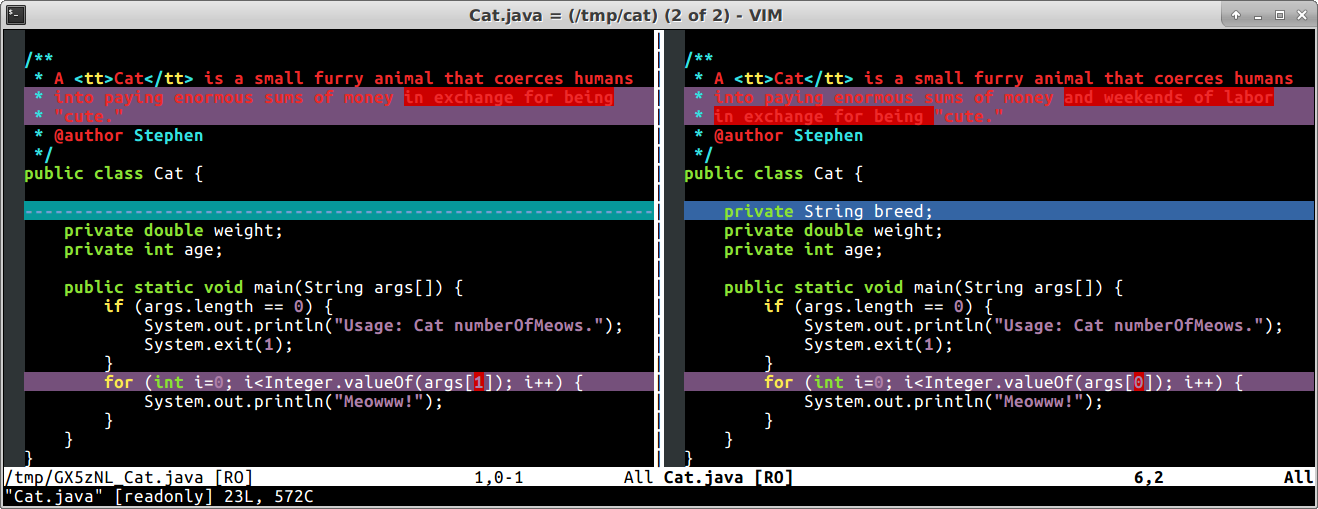
\includegraphics[width=1.1\textwidth]{catDiff.png}
\vspace{-.05in}
\caption{Using ``\texttt{git difftool}'' when configured with ``\texttt{vimdiff}''.}
\label{fig:catDiff}
\end{figure}

\index{cat.java@\texttt{Cat.java}}
Figure~\ref{fig:catDiff} shows what \texttt{vimdiff} looks like when you run
it. Its vertically-split pane shows two versions of the same file, with the
differences between the two in various colors. It is plain from the figure
that the differences between the two \texttt{Cat.java} versions are:

\index{javadoc@\texttt{javadoc}}
\begin{compactenum}
\item The JavaDoc class comment (see Chapter~\ref{ch:api}) has an extra phrase.
\item A new ``\texttt{breed}'' inst var has been added.
\item A bug has been fixed by changing the ``\texttt{args[1]}'' in the
\texttt{for} loop to ``\texttt{args[0]}''.
\end{compactenum}

Super cool, and easy to see at a glance. Learn to use this often in your
debugging and other code base investigations.

Don't attempt to use \texttt{vimdiff} to \textit{edit} your file, though. If
you're comparing two versions of a file and find a mistake, quit out of
\texttt{vimdiff} and enter plain-ol' \texttt{vim} to fix it. (Incidentally, to
quit \texttt{vimdiff} you have to enter ``\texttt{:q}'' \textit{twice}, once
for each of the panes. Sometimes it's quicker to use the ``\texttt{:qa}'' (for
``quit all'') sequence instead.)

\subsubsection{Specifying the versions to compare}

Okay. So that's how \texttt{vimdiff} (which is triggered from \texttt{git
difftool}) works in general. Now, how do you specify what versions of the
files you want to compare?

If you just type the command with no other arguments:

\begin{Verbatim}[fontsize=\small,samepage=true,frame=none]
$ git difftool
\end{Verbatim}

\index{workspace}
you'll be comparing \textit{your workspace} (yellow oval) against \textit{your
staging area} (purple diamond). This shows you the things that you have
changed \textit{since your last \texttt{git add}}. This is useful when asking,
``I'm about to do a commit...have I forgotten anything I meant to include?''

\index{staged@\texttt{-{}-staged} argument}
If you add the ``\texttt{-{}-staged}'' argument:

\begin{Verbatim}[fontsize=\small,samepage=true,frame=none]
$ git difftool --staged
\end{Verbatim}

\index{staging area}
\index{repository@``repo'' (repository)}
you'll be comparing \textit{your staging area} (purple diamond) with the
\textit{repo} (green box). This is useful when asking, ``if I do a commit
right now, exactly what changes will be recorded?''

\index{commit hash}
\index{hash}
Finally, to compare \textit{any two versions}, include the first few letters
of the commit hash of each. For instance, this command:

\begin{Verbatim}[fontsize=\small,samepage=true,frame=none]
$ git difftool bdb0fa3 7813b19
\end{Verbatim}

\index{Filbert}
will examine the changes Filbert made when he added multi-hairball support.
(Refer to the commit hashes in the \texttt{git log} output, above.) The first
hash identifies the commit Filbert was working with when he began making
changes (\textit{i.e.}, the one he started with), and the second is the hash
of the commit he himself made (the one he ended with). This process gives us
fine-grained resolution in examining the past and identifying errors.

% Rolling back to a previous version (git checkout)


\subsection{Using \texttt{git} with more than one human}

In a team environment, the \texttt{git} tool works much the same way, but with
an added level of complexity to ``join'' the developers together. Look at the
revised picture in Figure~\ref{fig:teamGit}.

\begin{figure}
\centering
\includegraphics[width=1.1\textwidth]{teamGit.pdf}  % 700x550
\caption{A development team's repos and workspaces.}
\label{fig:teamGit}
\end{figure}

\index{Betty Lou}
\index{github}
\index{BitBucket}
We now have two developers working on this feline program: Filbert and his
colleague Betty Lou. The picture is considerably more complex. First, notice
that the three salmon-colored squares represent \textit{different machines}
which communicate only over the Internet. Filbert and Betty Lou each have
their own laptop to do development on. And in addition, there is a third
machine involved: a publicly-available hosting service like BitBucket,
SourceForge, or github. Think of this public repo as the team's ``home base'':
despite the fact that at any given moment Filbert and Betty Lou may be writing
new code for the project, the latest stable version is always available in the
repo.

There are also some new \texttt{git} verbs we need to learn about to make this
picture work. To wit:

\begin{itemize}
\index{git@\texttt{git}!\texttt{git clone}}
\item \texttt{git clone}: Normally, the way this whole process kicks off is
that someone creates the initial version of the repo on github, and the other
team members \textbf{clone} copies of it. ``Clone'' is exactly what it sounds
like: it means to make an exact duplicate.

\index{git@\texttt{git}!\texttt{git push}}
github makes it easy to do this in a variety of ways. Perhaps the most common
is when one developer starts with an embryonic version of the code base,
creates his/her own local git repo, and then ``pushes'' (see below) this to a
new github project. It's also possible to start on github with a brand-new
blank project. At the time of this writing, a very helpful and obvious green
``New'' button is present on the github main account screen, with instructions
to follow for each of these different starting techniques.\footnote{Services
like github and BitBucket are free to use, by the way, as long as you keep
your repo public and visible to the world. The idea is that they're trying to
promote open source software, so in exchange for sharing your ideas, they're
giving you free storage space and tools. Some services even have free private
repos, sometimes in exchange for viewing ads.}

On the github project page, you'll see a button that says ``Clone or
download,'' and which will display a specific URL to your project if you click
on it. Then, on your local machine, you can go to the directory you want to be
the parent of your project, and type something like:

\begin{Verbatim}[fontsize=\small,samepage=true,frame=none]
$ git clone https://github.com/stuff/projectName.git projectName
\end{Verbatim}

which will populate your filesystem with a copy of all the repo's files.

\pagebreak
\index{git@\texttt{git}!\texttt{git push}}
\item \texttt{git push}: As usual, you'll constantly be making your own local
commits to your own copy of the repo as you work. You should do this every
time you reach a stopping point.

A new operation in the team environment is the ``\texttt{git push}''. It says
``take the updated contents of my own local repo (which have already been
committed) and propagate them up to the team repo in github.'' This is how you
share your changes with your teammates.

\index{git@\texttt{git}!\texttt{git commit}}
\index{commit}
Rule of thumb: making a local \texttt{commit} should be a common operation.
Doing a \texttt{push}, on the other hand, is rarer: you only do it when your
teammates need your latest code, and when your code is stable enough to
warrant making it ``the new normal'' in the team repo.

Last thing on \texttt{git push}: you normally don't do a \texttt{push} until
\textit{after} doing a \texttt{pull} to make sure you have your teammate's
latest code integrated in yours. See next bullet.

\index{git@\texttt{git}!\texttt{git pull}}
\item \texttt{git pull}: The inverse process of \texttt{push} is
\texttt{pull}. It means, ``go to github, fetch whatever changes have been made
by my fellow developers, and integrate them into my repo so I have the latest
and greatest.''

Now here's where \texttt{git} is fancy, and dare I say, seemingly magic.
Suppose you've been editing code for the project at the same time your
teammates are, and furthermore you're actually editing \textit{the same
files}. Doesn't that seem like it would be a nightmare? Doesn't it seem like
you would each be making incompatible changes, and that one person's work is
ultimately doomed to be wiped out by the other person's changes?

\index{merge}
\index{git@\texttt{git}!auto-merge}
That fear is indeed true if you're thinking of your code ``a file at a time.''
But \texttt{git} is smart enough to consider your code ``a \textit{line} at a
time.'' So if Filbert and Betty Lou are both making changes to
\texttt{Hairball.java}, but they're working on \textit{different parts} of
that file, it turns out that git can automatically and intelligently
\textbf{merge} the changes without you even having to worry about it.

When you do a \texttt{git pull} operation, \textit{read the output carefully.}
About 95\% of the time, it will give you happy messages like this:

\begin{Verbatim}[fontsize=\small,samepage=true,frame=none]
Auto-merging Hairball.java
Merge made by the 'recursive' strategy.
 Hairball.java | 1 +
 1 file changed, 1 insertion(+)
\end{Verbatim}

This is git's way of saying, ``your teammate was editing the same file(s) as
you, but it's chill; I figured out how to put their changes into your copy
without messing up anything you were doing.'' When this first happened to me,
I admit I was fearful, and couldn't comprehend how it could really be smart
enough to integrate those changes without me checking. But I've since learned
to stop worrying and love the bomb, and it really is ``all good.''

The other 5\% of the time, you're not so lucky, and you'll get a sad message
that says:

\begin{Verbatim}[fontsize=\small,samepage=true,frame=none]
Auto-merging Hairball.java
CONFLICT (content): Merge conflict in Hairball.java
Automatic merge failed; fix conflicts and then commit the result.
\end{Verbatim}

\index{conflict}
\index{git@\texttt{git}!conflict}
This situation is called a \textbf{conflict} and essentially means that you
and your teammate were working in the same \textit{part} of the file and made
incompatible changes. Perhaps one of you changed line 57 in one way, and the
other of you changed line 57 in a different way. Or perhaps one of you changed
line 90, while the other completely deleted lines 85-95. In these cases, git
can't figure out what you want to do, so it throws it back to you and asks you
to manually resolve it.

Resolving it is generally pretty easy. You open up the offending file(s) in
\texttt{vim}, and look for the markers ``$<<<<<$'', ``$=====$'', and
``$>>>>>$''. Here's the kind of thing you'll see:

\begin{Verbatim}[fontsize=\small,samepage=true,frame=single]
...
<<<<<<< HEAD
 * <tt>Cats</tt> are wonderful creatures that make good 
 * house pets.
=======
 * A <tt>Cat</tt> is a small fuzzy animal that coerces humans
 * into paying enormous sums of money and weekends of labor
 * in exchange for being "cute."
>>>>>>> c6812dcd33b977de0e7f0e9cab1eb1376bcfda88
...
\end{Verbatim}

Here's how to decipher that. The lines between the ``$<<<<<$ \texttt{HEAD}''
and the ``$=====$'' are what \textit{you} had in your version of the file. In
this example, you changed the \texttt{Cat} class JavaDoc entirely by rewriting
it in a more feline-friendly way. Meanwhile, your teammate (whose code is
marked between the ``$=====$'' and the ``$>>>>>$ \texttt{c6812...}'') made a
smaller change to that comment, changing ``furry'' to ``fuzzy.'' All that
matters now is what you want to do about these changes. It's your job as a
developer to restore that part of the \texttt{Cat.java} file to be
\textit{what your team wants the code to look like moving forward.} Perhaps
you keep your change, perhaps you keep your teammate's, perhaps it's a
combination of both. But after fixing it up the way it should be (with maybe a
phone call or chat session with your colleague to make sure you're on the same
page), you will have removed the ``$<<<<<$'' and ``$=====$'' and ``$>>>>>$''
markers and can ``\texttt{git add}'' and commit your changes. Finally, you can
then push the combined changes to the team repo, and everything goes on hunky
dory.

Normally, the only time you end up in the 5\% conflict case (instead of the
95\% auto-merge case) is when you and your teammates aren't communicating well
(or enough). Two developers both editing the same lines of code and not
realizing that the other person is doing it is usually a sign that you need to
work more closely together or be more explicit about who's working on what. A
simple email or text often does the trick.

\end{itemize}

Bottom line: using the \texttt{git} verbs \texttt{add}, \texttt{commit},
\texttt{pull}, and \texttt{push} properly is your key to ensuring your team
has a living, breathing, healthy, working repository of shared code.

Here are the most common pitfalls I see:

\index{git@\texttt{git}!\texttt{git push}}
\index{git@\texttt{git}!\texttt{git pull}}
\index{git@\texttt{git}!\texttt{git stash}}
\index{man@\texttt{man}}
\begin{compactitem} \item Forgetting to do a \texttt{pull} before trying a
\texttt{push}. git won't allow you to \texttt{push} into a repo if you're
out-of-date. You must first \texttt{pull} the recent changes so you're all in
sync, and \textit{then} you can \texttt{push} your new changes to it. \item
Forgetting to do a local \texttt{commit} before trying to \texttt{pull}. git
won't let you pull changes from another repo if you have car parts all over
your own garage. Make sure you check everything in and have a clean local
workspace before doing that.\footnote{An alternative to a full local commit
here is the ``\texttt{git stash}'' command which I've found useful. Doing a
``\texttt{stash}'' is different than a \texttt{commit}, since you're not
actually marking version control with labeled changes. Instead, you're sort of
sweeping stuff under the rug to make your workspace temporarily clean, for the
sake of doing an important \texttt{pull} operation from your teammates. You
can then pull your stuff back out from under your rug and continue. For
details, type ``\texttt{man git stash}'' and read carefully.}

\end{compactitem}


